\providecommand{\main}{../..}
\documentclass[\main/thesis.tex]{subfiles}
\begin{document}

\section{The Next Numeral}\label{next}

Paul Benacerraf once argued\cite{benacerraf1965numbers} that, there are two kinds
of \textit{counting} which correspond to \textbf{transitive} and \textbf{intransitive}
uses of the verb ``to count.'' Transitive counting, in his sense, is to assign one
of the numbers to the cardinality of a set, by establishing a one-to-one correspondence
between the numbers and the objects one is counting, all the way from none to
all. Intransitive counting, on the other hand, is to generate a sequence of
notation, that could go as far as we need. And it seems that one can only learn
how to count intransitively first, before knowning how to count transitively,
but not vice versa. So it is important to know how to generate the next numeral
we need.

\subsection{What does it mean by ``The Next''?}

When mapping some systems such as {\lstinline|Numeral 10 5 0|} onto
the natural numbers, their number lines appear to be ``gapped'' because their
evaluations are not \textit{surjective}.
The number ``6'', for example, has no correspondence on the numeral side.

\begin{center}
    \begin{adjustbox}{max width=\textwidth}
        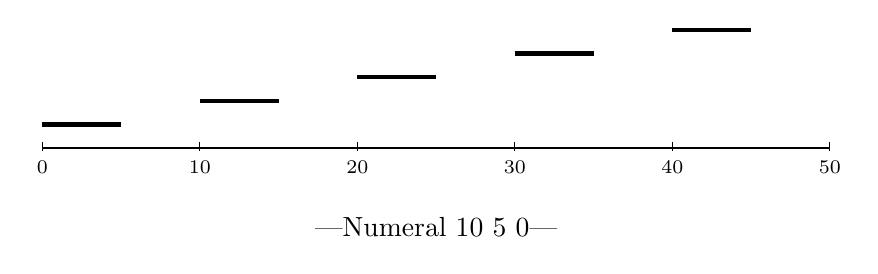
\begin{tikzpicture}
            % a straight line segment
            \draw (0, 0) -- (10, 0);
            % the ticks and their labels
            \foreach \x  in {0,...,5}
                \draw[xshift=\x*2 cm] (0pt,2pt) -- (0pt,-1pt) node[below,fill=white] {\scriptsize\the\numexpr\x*10\relax};
            \foreach \x  in {0,...,4}
                \draw[ultra thick, xshift=\x*2 cm, yshift=\x*0.3 cm] (0,0.3) -- (1,0.3);
            % labels
            \node at (5, -1) {{\lstinline|Numeral 10 5 0|}};
        \end{tikzpicture}
    \end{adjustbox}
\end{center}

Whilst systems such as {\lstinline|Numeral 10 15 0|} map more than one numeral
onto the same number. We can see immediately that their evaluations are not
\textit{injective} as those number lines ``overlap'' with each other.

\begin{center}
    \begin{adjustbox}{max width=\textwidth}
        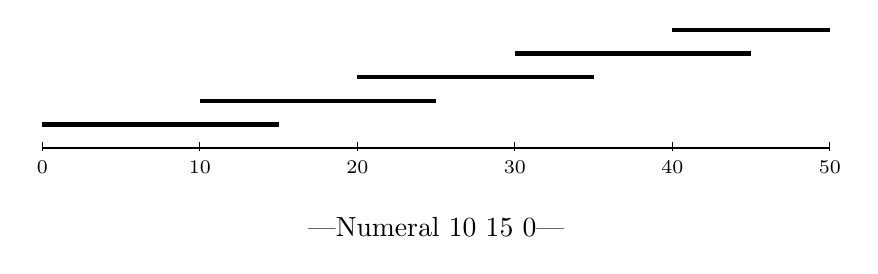
\begin{tikzpicture}
            % a straight line segment
            \draw (0, 0) -- (10, 0);
            % the ticks and their labels
            \foreach \x  in {0,...,5}
                \draw[xshift=\x*2 cm] (0pt,2pt) -- (0pt,-1pt) node[below,fill=white] {\scriptsize\the\numexpr\x*10\relax};
            \foreach \x  in {0,...,3}
                \draw[ultra thick, xshift=\x*2 cm, yshift=\x*0.3 cm] (0,0.3) -- (3,0.3);
            \draw[ultra thick, xshift=8 cm, yshift=1.2 cm] (0,0.3) -- (2,0.3);
            % labels
            \node at (5, -1) {{\lstinline|Numeral 10 15 0|}};
        \end{tikzpicture}
    \end{adjustbox}
\end{center}

As we can see, numerals do not align with numbers perfectly.
Finding ``the next number'' thus becomes a non-trivial problem.
Therefore, we define the next numeral as \textbf{the least numeral that is greater than itself}.

\subsection{Implementation}

Given a numeral, say {\lstinline|xs|}, to find the next numeral of {\lstinline|xs|},
it sensible to expect that {\lstinline|xs|} must not be a maximum.
Otherwise, there exists no such a numeral that is \textit{greater than itself}.

Again, the indices are classified by {\lstinline|numView|} into four categories.
The case {\lstinline|NoDigits|} and {\lstinline|AllZeros|} of are rather trivial.
We focus on the other two.

\begin{lstlisting}
next-number : ∀ {b d o}
    → (xs : Numeral b d o)
    → ¬ (Maximum xs)
    → Numeral b d o
next-number {b} {d} {o} xs ¬max with numView b d o
next-number xs ¬max | NullBase d o = ?
next-number xs ¬max | NoDigits b o = NoDigits-explode xs
next-number xs ¬max | AllZeros b   =
    contradiction (Maximum-AllZeros xs) ¬max
next-number xs ¬max | Proper b d o proper = ?
\end{lstlisting}

\subsection{Validating the Implementation}

To validate the correctness of the implementation of {\lstinline|next-number|},
i.e., to make sure that the function does return a numeral that is:

\begin{enumerate}
    \item greater than the given numeral
    \item the least of all such numerals
\end{enumerate}

We need to prove these two propositions:

\begin{lstlisting}
next-number-is-greater : ∀ {b d o}
    → (xs : Numeral b d o)
    → (¬max : ¬ (Maximum xs))
    → ⟦ next-number xs ¬max ⟧ > ⟦ xs ⟧
\end{lstlisting}

\begin{lstlisting}
next-number-is-immediate : ∀ {b d o}
    → (xs : Numeral b d o)
    → (ys : Numeral b d o)
    → (¬max : ¬ (Maximum xs))
    → ⟦ ys ⟧ > ⟦ xs ⟧
    → ⟦ ys ⟧ ≥ ⟦ next-number xs ¬max ⟧
\end{lstlisting}

We come up with the name ``immediate''
because ``the least numeral that is greater than itself'' is a bit too wordy.

\subsection{Outline}

We are going to finish programs and proofs of systems of {\lstinline|NullBase|}
and {\lstinline|Proper|} respectively.

\begin{itemize}
    \item {\lstinline|NullBase|}
        \begin{enumerate}
            \item {\lstinline|next-number-NullBase|}
            \item {\lstinline|next-number-is-greater-NullBase|}
            \item {\lstinline|next-number-is-immediate-NullBase|}
        \end{enumerate}
    \item {\lstinline|Proper|}
        \begin{itemize}
            \item {\lstinline|next-number-Proper|}
            \item {\lstinline|next-number-is-greater-Proper|}
            \item {\lstinline|next-number-is-immediate-Proper|}
        \end{itemize}
\end{itemize}

However, programs and proofs of systems of {\lstinline|Proper|} will be defined
\textit{simultaneously} with mutually recursive definitions.
The reason why we need properties like {\lstinline|next-number-is-greater-Proper|}
and {\lstinline|next-number-is-immediate-Proper|} in the first place is that
they are neccessary for implementing {\lstinline|next-number-Proper|}.

\subsection{The Next Numeral of NullBase}

To find the next numeral of systems of {\lstinline|NullBase|},
all we have to do is to manipulate the LSD.
Since only the value of the LSD has effect on the evaluation.
All numerals are mapped onto this single and continuous number line below.

\begin{center}
    \begin{tikzpicture}
        % a straight line segment
        \draw (0, 0) -- (10, 0);
        % the ticks and their labels
        \draw[xshift=0cm] (0pt,2pt) -- (0pt,-1pt) node[below,fill=white] {\the\numexpr0};
        % the thicker segment
        \draw[ultra thick] (1,0) -- (9,0);
        % the labels
        \node[fill=black,draw=black,circle,inner sep=2pt,label=above:{$o$}] at (1,0) {};
        \node[fill=black,draw=black,circle,inner sep=2pt,label=above:{$d+o$}] at (9,0) {};
        \node at (5, -0.5) {{\lstinline|ℕ|}};
    \end{tikzpicture}
\end{center}

Finding the next numeral is as simple as incrementing the LSD.
To make room for the increment, numerals that are mapped onto the rightmost
number of the line are excluded because they also happen to be maxima.

\begin{center}
    \begin{tikzpicture}
        % a straight line segment
        \draw (0, 0) -- (10, 0);
        % the ticks and their labels
        \draw[xshift=0cm] (0pt,2pt) -- (0pt,-1pt) node[below,fill=white] {\the\numexpr0};
        % the thicker segment
        \draw[ultra thick] (1,0) -- (8,0);
        % inner nodes
        \foreach \x in {2,...,7}
            \node[fill=black,draw=black,circle,inner sep=2pt](\x) at (\x,0) {};
        % labels
        \node[fill=black,draw=black,circle,inner sep=2pt,label=above:{$o$}](1) at (1,0) {};
        \node[fill=black,draw=black,circle,inner sep=2pt,label=above:{$d+o-1$}](8) at (8,0) {};
        \node[fill=white,draw=black,circle,inner sep=2pt,label=below:{$d+o$}](9) at (9,0) {};
        \node at (5, -1) {{\lstinline|ℕ|}};

        \foreach \x in {1,...,8} {
            \pgfmathsetmacro{\y}{\x + 1}
            \path[->,>=stealth']
                (\x) edge[bend right=60,transform canvas={xshift=-1pt, yshift=-3pt}] node [left] {} (\y);
        };
    \end{tikzpicture}
\end{center}

\subsubsection{A View within another}

Although the system {\lstinline|Numeral 0 1 0|} is classified as {\lstinline|NullBase|}
rather than {\lstinline|AllZeros|} by the view function {\lstinline|numView|}
because of the order of pattern matching.
{\lstinline|Numeral 0 1 0|} still retain characteristics of {\lstinline|AllZeros|},
making it an outlier among other systms of {\lstinline|NullBase|}.

To handle this, we further classify the indices of {\lstinline|NullBase|} into
two subcategories with a view.

\begin{lstlisting}
data NullBaseView : (d o : ℕ) → Set where
    AllZeros : NullBaseView 0 0
    Others   : ∀ {d o}
             → (bound : d + o ≥ 1 ⊔ o)
             → NullBaseView d o

nullBaseView : ∀ d o → NullBaseView d o
nullBaseView = ...
\end{lstlisting}

The sole purpose of this view is to isolate {\lstinline|Numeral 0 1 0|} from
all the other systems of {\lstinline|NullBase|}.

\subsubsection{The Function}


Systems are first classified by {\lstinline|nullBaseView|} into {\lstinline|Numeral 0 1 0|}
and the others.

\begin{lstlisting}[basicstyle=\ttfamily\scriptsize]
next-number-NullBase : ∀ {d o}
    → (xs : Numeral 0 (suc d) o)
    → ¬ (Maximum xs)
    → Numeral 0 (suc d) o
next-number-NullBase {d} {o} xs ¬max with nullBaseView d o
\end{lstlisting}

\paragraph{AllZeros}

Every numeral of {\lstinline|Numeral 0 1 0|} is a maximum, which contradicts
with the assumption that the given numeral is not a maximum.

\begin{lstlisting}[basicstyle=\ttfamily\scriptsize]
next-number-NullBase xs       ¬max | AllZeros =
    contradiction (Maximum-AllZeros xs) ¬max
\end{lstlisting}

\paragraph{Others}

First, rule out the numerals with the greatest LSD hence the maxima.
Next, increment rest of the numerals with {\lstinline|digit+1|}.

\begin{lstlisting}[basicstyle=\ttfamily\scriptsize]
next-number-NullBase xs       ¬max | Others _ with Greatest? (lsd xs)
next-number-NullBase xs       ¬max | Others _ | yes greatest =
    contradiction (Maximum-NullBase-Greatest xs greatest) ¬max
next-number-NullBase (x ∙   ) ¬max | Others _ | no ¬greatest =
    digit+1 x ¬greatest ∙
next-number-NullBase (x ∷ xs) ¬max | Others _ | no ¬greatest =
    digit+1 x ¬greatest ∷ xs
\end{lstlisting}

\subsubsection{next-number-is-greater-NullBase}

\begin{lstlisting}[basicstyle=\ttfamily\scriptsize]
next-number-is-greater-NullBase : ∀ {d o}
    → (xs : Numeral 0 (suc d) o)
    → (¬max : ¬ (Maximum xs))
    → ⟦ next-number-NullBase xs ¬max ⟧ > ⟦ xs ⟧
next-number-is-greater-NullBase {d} {o} xs ¬max with nullBaseView d o
next-number-is-greater-NullBase xs ¬max | AllZeros =
    contradiction (Maximum-AllZeros xs) ¬max
next-number-is-greater-NullBase xs ¬max | Others _ with Greatest? (lsd xs)
next-number-is-greater-NullBase xs ¬max | Others _ | yes greatest =
    contradiction (Maximum-NullBase-Greatest xs greatest) ¬max
next-number-is-greater-NullBase {d} {o} (x ∙) ¬max | Others _ | no ¬greatest =
    start
        suc ⟦ x ∙ ⟧
    ≈⟨ refl ⟩
        suc (Digit-toℕ x o)
    ≈⟨ sym (digit+1-toℕ x ¬greatest) ⟩
        Digit-toℕ (digit+1 x ¬greatest) o
    ≈⟨ refl ⟩
        ⟦ digit+1 x ¬greatest ∙ ⟧
    □
next-number-is-greater-NullBase {d} {o} (x ∷ xs) ¬max | Others _ | no ¬greatest =
    start
        suc ⟦ x ∷ xs ⟧
    ≈⟨ refl ⟩
        suc (Digit-toℕ x o) + ⟦ xs ⟧ * 0
    ≈⟨ cong (λ w → w + ⟦ xs ⟧ * 0) (sym (digit+1-toℕ x ¬greatest)) ⟩
        Digit-toℕ (digit+1 x ¬greatest) o + ⟦ xs ⟧ * 0
    ≈⟨ refl ⟩
        ⟦ digit+1 x ¬greatest ∷ xs ⟧
    □
\end{lstlisting}

\subsection{The Next Numeral of Proper}

% Revisit the view function {\lstinline|numView|}.
% First, it pattern matches on {\lstinline|d|}, excluding systems with no digits;
% and then on {\lstinline|b|}, exluding systems with bases of $ 0 $.
% There is an order of pattern matching on the three indices.
%
\end{document}
